% !TEX root = ./main.tex

\chapter{Implementierung}

Diese Thesis setzt sich aus Unterprojekten zusammen, die eine gemeinsame Pipeline zum Training eines Neuronalen Netzes vollenden: die Datengenerierung, das Identifizieren und Entzerren einer Dartscheibe und die Lokalisierung von Pfeilspitzen in entzerrten Bildern. Die Implementierungen dieser Projekte wird in diesem Abschnitt genauer beleuchtet. Als erster Teil der Pipeline wird die Datenerstellung in \autoref{sec:impl:daten} betrachtet, danach wird in \autoref{sec:impl:cv} auf die Identifizierung und Entzerrung der Dartscheibe in Bildern eingegangen und abschließend wird in \autoref{sec:impl:ki} darauf eingegangen, wie diese Daten zum Trainieren eines Neuronalen Netzes genutzt werden mit dem Ziel, die erzielte Punktzahl und die Positionen der Dartpfeile anhand einzelner Bilder zu identifizieren.

% -------------------------------------------------------------------------------------------------
% DATENGENERIERUNG
\section{Datengenerierung}
\label{sec:impl:daten}

Die Datengrundlage für dieses Projekt setzt sich aus unterschiedlichen Quellen zusammen. Neben bereits annotierten Daten des Deepdarts-Systems von \citeauthor{deepdarts} \cite{deepdarts-data} und manuell aufgenommenen Daten besteht der weitaus größte und für das Training des Neuronalen Netzes relevanteste Teil aus gerenderten und damit nicht realen Daten. Der Hintergrund dieser Entscheidung liegt in der fehlerbehafteten Datengrundlage der bereits vorhandenen Daten des Deepdarts-Systems.

Den Daten des Deepdarts-Systems liegen einige Fehlstände zugrunde, die in dieser Thesis aufgegriffen und verbessert werden sollten. Zum einen sind die Daten durch die manuelle Aufnahme wenig variabel, begründet darin, dass durch reale Aufnahmen nur bedingt viele Umgebungen abgedeckt werden können. Allem voran sind die Wahl der Dartscheibe, die Aufnahmeparameter der Kamera und die Spanne an Belichtungsmöglichkeiten Variablen, die durch die manuelle Aufnahme von Bildern stark beschränkt und nur schwer zu realisieren sind. Zum anderen beherbergen manuelle Aufnahmen der Risiko der fehlerhaften Kennzeichnung von Gegebenheiten und Einbringung ungewollter Verzerrungen. So kann es durch manuelles Annotieren passieren, dass Pfeilspitzen nicht korrekt identifiziert werden und damit fehlerhafte Daten zum Trainieren des Neuronalen Netzes verwendet werden.

Die synthetische Datenerstellung dieser Thesis basiert auf der 3D-Modellierungssoftware \textit{Blender}\cite{blender}. Mit dieser ist die Erstellung fotorealistischer und parametrisierbarer Szenen möglich, die gepaart mit externen Skripten zur automatisierten Datenerstellung genutzt wird. Dazu wird eine Szene erstellt, die als Blaupause aller synthetischer Daten fungiert. Die Objekte und Gegebenheiten in dieser Szene werden durch externes Setzen von spezifischen Parametern gelenkt und ermöglicht die Simulation einer Vielzahl unterschiedlicher Szenarien und Umgebungsbedingungen.

% ------------------------------------------------------------------------

\subsection{Die Szene in Blender}
\label{sec:impl:daten:blender}

Das zentrale Objekt der Datenerstellung ist die 3D-Szene an sich. Sie bildet die Grundlage sowohl zur Auswertung der Entzerrung als auch aller Trainingsdaten des Neuronalen Netzes. Die Handhabung dieser Szene geht daher mit großer Sorgfalt einher. Die Szene setzt sich aus unterschiedlichen Bestandteilen zusammen, in die Kategorien \textit{Parametrisierung}, \textit{Hauptobjekte} und \textit{Nebenobjekte}. Auf diese wird in den folgenden Unterabschnitten eingegangen.


% -----------------------------------------------
\subsubsection{Parametrisierung}
\label{sec:impl:daten:blender:parameter}

Bevor auf die Objekte und ihre Eigenschaften eingegangen wird, ist die Klärung der Parametrisierung der Szene relevant. Die Zusammensetzung, Geometrie und Texturierung der Objekte in der Szene basiert auf der globalen Szenenzeit $t_S \in [0, 2^{15}]$. Dieser Parameter wird von den Objekten als Seed zur Generierung von Zufallsvariablen genutzt, die das jeweilige Aussehen beeinflussen. Neben diesem Faktor steht darüber hinaus ein Altersfaktor $a \in [0, 1]$ zur Beeinflussung des Alters der Dartscheibe zur Verfügung. Dieser Faktor ist spezifisch dazu vorgesehen, Variablen zwischen \quotes{alten} und \quotes{neuen} Werten zu skalieren, sodass mit einem geringen Altersfaktor neue, unbeschädigte Dartscheiben generiert werden, wohingegen mit einem hohen Altersfaktor Dartscheiben generiert werden, die starke Abnutzungen und Verfärbungen aufweisen. Die Magnitude dieses Faktors steht dabei in nicht-linearer Abhängigkeit zur Szenenzeit, wie in \autoref{fig:age} dargestellt. Mit dieser Nichtlinearität wird eine heuristische Gewichtung zwischen neuen und alten Dartscheiben erzielt.

\begin{center}
    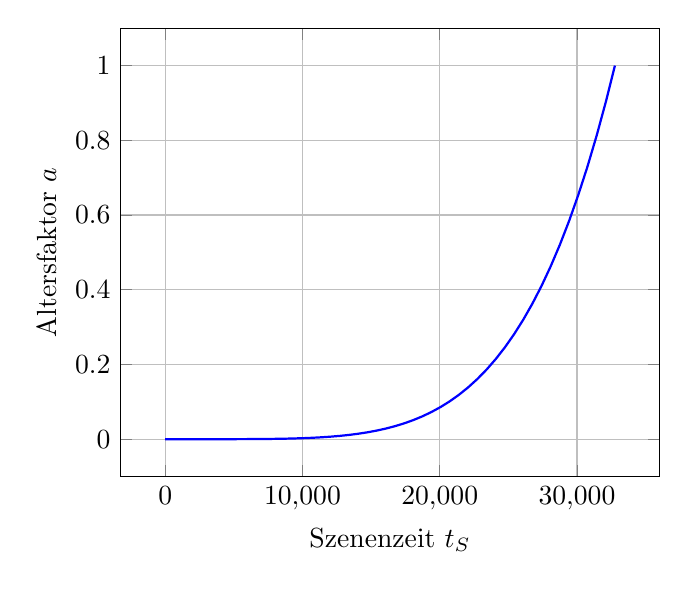
\begin{tikzpicture}
        \begin{axis}[
                ymin = -0.1,
                ymax=1.1,
                domain = 0:32768,
                samples=50,
                xlabel={Szenenzeit $t_S$},
                ylabel={Altersfaktor $a$},
                scaled x ticks = false,
                grid=both,
            ]
            \addplot[thick,blue]{(x/32768)*(x/32768)*(x/32768)*(x/32768)*(x/32768)};
        \end{axis}
    \end{tikzpicture}
    \captionof{figure}{Abhängigkeit des Altersfaktors $a$ von der Szenenzeit $t_S$ für die Datengenerierung.}
    \label{fig:age}
\end{center}

Die Verwendung der Parameter ist je nach Objekt unterschiedlich; während sie in Hauptobjekten häufig eingesetzt werden, nutzen Nebenobjekte diese eher selten. Dies liegt im Zusammenhang mit der Häufigkeit ihres Vorkommens in den Daten und damit der Notwendigkeit ihrer Variabilität.


% -----------------------------------------------
\subsubsection{Hauptobjekte}
\label{sec:impl:daten:blender:hauptobjekte}

% Als \textit{Hauptobjekte} werden diejenigen Objekte in der Szene beschrieben, die zentral für die Datenerstellung sind. Namentlich sind dies die Dartscheibe, die Dartpfeile und die Kamera, gepaart mit der Komposition.

\paragraph{Dartscheibe}
\label{sec:impl:daten:blender:hauptobjekte:dartscheibe}

% Die Dartscheibe ist das komplexeste Objekt der Szene, da ihr Erscheinungsbild als zentrales Element der Bilder ausschlaggebend für die Komplexität und Variabilität der Daten ist. Aus diesem Grund ist sie mit einer Vielzahl an Parametern und Eigenschaften versehen. Sie ist gemäß der Richtlinien \quotes{Playing and Tournament Rules} der \ac{WDF} \cite{wdf-rules} erstellt. Dieses Regelwerk legt die Dimensionen und Abstände der Felder sowie etwaige Toleranzen fest. Auf dieses Regelwerk wurde sich in dieser Thesis bei der Arbeit mit Dartscheiben orientiert, Abweichungen durch esoterische Maße und Erscheinungsbilder von Dartscheiben, die nicht durch dieses Regelwerk gestützt sind, werden für diese Arbeit nicht in Betracht gezogen. Die Parametrisierung der Scheibe ist in zwei Bereiche einzuteilen: Geometrie und Textur.

% Die Geometrie der Dartscheibe ist durch die Regeln der \ac{WDF} zu großen Teilen vorgegeben. Um Alter und Abnutzung der Dartscheibe zu simulieren, wird der Deformationsgrad der Spinne\footnote{Als Spinne werden die Abgrenzungen zwischen den Feldern bezeichnet.} beeinflusst.
Dazu wird der Parameter $t_S$ als Seed für eine 2D-Verschiebung der Mesh-Vertices anhand einer zusammenhängenden Noise-Textur verwendet und diese wird mit dem Parameter $a$ in ihrer Stärke moduliert. Dadurch weisen Dartscheiben mit einem hohen Altersfaktor $a$ eine größere Deformierung der Spinne auf während Dartscheiben mit einem geringen Wert von $a$ geringe bis keine Deformierung aufweisen. Ebenfalls von dem Altersfaktor beeinflusst wird die Art der Spinne: Während Spinnen neuer Dartscheiben aus dünnen Drähten bestehen, ist der Durchmesser dieser bei alten Dartscheiben größer und die Wahrscheinlichkeit steigt, dass die Spinne mit weiteren Drähten zur Befestigung der Spinne auf der Scheibe versehen ist.

Der Großteil der variablen Parameter der Dartscheibe liegt jedoch nicht in der Geometrie, sondern in dem Material der Dartscheibe. Anhand unterschiedlicher Zufallsverteilungen, gestützt durch $t_S$ als Seed, werden die Farben der Felder, Abnutzung der Scheibe und Anzahl der Einstichlöcher im Sisal bestimmt.
Um realistische Materialien zu simulieren, werden unterschiedliche Imperfektionen in das Material eingearbeitet. Diese lassen sich in zwei Kategorien einteilen: Reine Farbänderungen und Farbänderungen, die eine Änderung der Normalen mit sich ziehen.

Zu der ersten Kategorie der Imperfektionen zählen kleine Haare und Staubpartikel, die sich auf der Dartscheibe ablagern. Diese sorgen für feine Verfärbungen und unterschiedliche Lichtbrechungen. Dazu kommen Spuren von Abnutzung, die je nach Alter unterschiedlich stark ausgeprägt sind. Diese Abnutzungen sind in Form von Kratzern und Abrissstellen in die Scheibe eingearbeitet.
Die zweite Kategorie der Imperfektionen sind Risse und Einstichstellen im Sisal. Durch seine Beschaffenheit reißt Sisal mit steigendem Alter. Diese Risse werden sowohl durch Farbänderung als auch durch Einkerbungen in den Feldern simuliert. Weiterhin werden Einstichlöcher von Dartpfeilen simuliert und farblich hervorgehoben. Diese Faktoren sind ebenfalls abhängig vom Alter der Dartscheibe unterschiedlich stark ausgeprägt.

Mit zunehmendem Altersfaktor $a$ nimmt weiterhin die Farbsättigung der schwarzen und weißen Felder zu, wohingegen rote und grüne Felder an Sättigung verlieren und dunkler werden. Diese Anpassung der Feldfarben simuliert das Altern des Sisals der Dartscheiben, basiert auf Beobachtungen neuer und alter Dartscheiben. Darüber hinaus weisen alte Dartscheiben häufiger abgenutzte Zahlenringe auf, die sich durch Rost und Verfärbungen auszeichnen.



\paragraph{Dartpfeile}
\label{sec:impl:daten:blender:hauptobjekte:dartpfeile}

Neben der Dartscheibe sind die Dartpfeile weitere Hauptobjekte. Im Gegensatz zur Dartscheibe ist ihre Geometrie weniger stark durch das Regelwerk der \ac{WDF} vorgegeben, sodass eine größere Variabilität geschaffen werden kann. Dartpfeile setzen sich aus den Bestandteilen \textit{Tip}, \textit{Barrel}, \textit{Shaft} und \textit{Flight} zusammen; für jedes dieser Teile existiert eine Gruppe an Objekten, die zufällig miteinander kombiniert und teilweise zufällig texturiert werden. Die unterschiedlichen Objekte der jeweiligen Klassen sind in \autoref{img:dartpfeil_teile} dargestellt. Diese Einzelteile sind inspiriert durch reale Dartpfeile. Bei dem Zusammensetzen werden Tip, Barrel und Shaft zufällig gestaucht oder gestreckt, um weitere Variabilität in die Dartpfeile zu integrieren. Für die Farben der Flights wird eine Basistextur zufällig gesampled. Zur Erstellung dieser Basistextur wurde die Bilderstellungs-KI von DeepAI genutzt \cite{deepai-image}. Zudem wird die Stärke der Verformung der Flights durch den Altersfaktor $a$ gesteuert: je älter ein Pfeil ist, desto stärker kann er deformiert sein. In \autoref{img:dart_examples} sind einige Beispiele verschiedener Dartpfeile dargestellt. Zu erkennen ist in diesen die zufällige Wahl der Bestandteile und die Variation der Materialien.

\begin{figure}
    \centering
    \includegraphics[width=\textwidth]{imgs/darts.png}
    \caption{Bestandteile der Dartpfeile (von links nach rechts): Tips, Barrels, Shafts und Flights.}
    \label{img:dartpfeil_teile}
\end{figure}

\begin{figure}
    \centering
    \includegraphics[width=0.7\textwidth]{imgs/darts_examples.png}
    \caption{Darts Examples}
    \label{img:dart_examples}
\end{figure}

\paragraph{Kamera und Komposition}
\label{sec:impl:daten:blender:hauptobjekte:kamera}

Ein weiterer wichtiger Bestandteil der Szene sind die Kamera und die Komposition. Das Zusammenspiel dieser Bereiche ist daran ausgerichtet, Bilder zu rendern, die in ihrem Aussehen an Aufnahmen von Mobiltelefonen angelehnt sind. Dabei werden Blurring, Bloom, Lens Distortion und Film Grain simuliert, um Ungenauigkeiten von Handyaufnahmen zu simulieren. Die jeweiligen Ausprägungen dieser Nachverarbeitungsschritte wurden durch Analyse eigener Aufnahmen unterschiedlicher Kameramodelle eingestellt. Der Fokuspunkt der Kamera ist auf ein Objekt gelegt, das zufällig im Bereich um die Dartscheibe platziert wird. Weitere interne und externe Kameraparameter wie Bewegungsunschärfe, Auflösung oder Brennweite werden bei der Erstellung durch Skripte gesetzt, die in \autoref{sec:impl:daten:python} erläutert werden.

% -----------------------------------------------
\subsubsection{Nebenobjekte}
\label{sec:impl:daten:blender:nebenobjekte}

Zusätzlich zu den Hauptobjekten, die in nahezu allen Bildern zu sehen sind, existieren in der Szene weitere Objekte die zufällig erscheinen können und die Szene variabler gestalten. Diese Objekte werden als Nebenobjekte bezeichnet und in den folgenden Unterkapiteln beschrieben.

\paragraph{Beleuchtung}
\label{sec:impl:daten:blender:nebenobjekte:licht}

Es werden unterschiedliche Arten der Beleuchtung eingesetzt. Dazu zählen Environment-Texturen, der Kamerablitz, ein Spotlight, Deckenlampen und ein LED-Ringlicht um die Dartscheibe herum. Die Environment-Texturen stammen von der Webseite PolyHaven\cite{polyhaven} und werden zufällig gewählt und in ihrer Intensität moduliert. Der Kamerablitz ist als helles Punktlicht modelliert, das wenige Zentimeter von der Kamera entfernt liegt. Dadurch ist eine realistische Ausleuchtung der Szene mit scharfem Schattenwurf in direkter Nähe der Objekte möglich. Weiterhin für scharfe Schatten sorgt ein Spotlight, das sich über der Kamera befindet und auf die Dartscheibe gerichtet ist. Diese Art der Beleuchtung wird im Strongbow's in Kiel verwendet, wo unter anderem Daten für diese Arbeit aufgenommen wurden. Deckenlampen wurden durch Leuchtstoffröhren in warmen Farbtönen in vergitterten Boxen modelliert, die in zwei Reihen entlang der Decke aufgereiht sind. Die Art der Beleuchtungen und ihre Ausprägungen werden nicht in der Szene festgelegt, sondern durch externe Skripte zur Erstellung und Randomisierung der Daten.

\paragraph{Dartschrank und LED-Ring}
\label{sec:impl:daten:blender:nebenobjekte:cabinet}

Um die Dartscheibe herum können ein Dartschrank oder ein LED-Ring eingeblendet werden. Der LED-Ring besteht aus einem Zylinderförmigen Korpus, an dessen Vorderkante auf die Dartscheibe gerichtete LED-Lichter angebracht sind. Dieses Art des Ringlichts ist geläufig bei der Verwendung von Dartscheiben; die Farbe der LEDs werden, ebenso wie die Farbe des Rings, zufällig gewählt. Der Dartschrank ist mit einer Holztextur versehen, deren Sättigung und Helligkeit ebenfalls zufällig gewählt wird, und die Türen werden in einem zufälligen Winkel geöffnet.

Beide Objekte können nicht gemeinsam auftreten, da sie im selben Raum agieren und ein gemeinsames Einblenden zu Überschneidungen der Objekte führen würde. Folglich ist entweder eines dieser Objekte oder keines vorhanden.

% ------------------------------------------------------------------------

\subsection{Python-Skript zur Randomisierung von Parametern}
\label{sec:impl:daten:python}

Das Rendern der Szene geschieht nicht aus Blender heraus, sondern wird durch die Python-Bibliothek \textit{bpy} gesteuert. Durch diese Bibliothek ist es möglich, die Szene deskriptiv und ohne GUI zu manipulieren und zu steuern. Das Setzen von Parametern und das gezielte Anordnen der Objekte in der Szene wird auf diese Weise erzielt.

\subsubsection{Generelles Setup}
\label{sec:impl:daten:python:setup}

Der erste Schritt zur Erstellung einer Szene für das Rendern eines Samples ist die Randomisierung des globalen Szenenparameters $t_S$. Dieser wird von den Objekten als Seed zur Erstellung von Zufallswerten und als Altersfaktor genutzt. Er wird uniform zwischen der minimalen und maximalen Szenenzeit gewählt.

\subsubsection{Beleuchtung und Umgebungsobjekte}
\label{sec:impl:daten:python:licht}

Die Beleuchtung der Szene ist ein mehrschrittiger Prozess, in dem eine Abstimmung der unterschiedlichen Beleuchtungsmöglichkeiten geschaffen wird, um eine realistische Verwendung von Lichtquellen zu erzielen. Der erste Schritt der Beleuchtung ist die Wahl der Umgebungsbeleuchtung durch die Environment-Textur. Diese wird zufällig aus einem Pool von $>200$ HDRIs und einer Intensität $I_{HDRI} \in [0, 1]$ gewählt. Zudem wird sie zufällig um die Z-Achse rotiert, um die Anzahl der Dopplungen gleicher Hintergründe weiter zu minimieren. Die Intensität $I_{HDRI}$ bestimmt die Wahrscheinlichkeit der Aktivierung von Kamerablitz, Spotlight und Deckenbeleuchtung. Je dunkler die Umgebung, desto wahrscheinlicher ist die Existenz weiterer Beleuchtungen.
Weiterhin wird mit einer Wahrscheinlichkeit von $5\%$ der Dartschrank eingeblendet und mit einer Wahrscheinlichkeit von $15\%$ das Ringlicht. Diese Fälle schließen sich gegenseitig aus, sodass lediglich eines von beiden Objekten existieren kann.
Sind weder Kamerablitz, Spotlight oder der LED-Ring aktiviert, ist die Deckenbeleuchtung gesichert als Rückfall-Lichtquelle aktiviert, um unbeleuchtete Szenen auszuschließen.

\subsubsection{Text}
\label{sec:impl:daten:python:text}

Um den Rand der Dartscheibe befinden sich zwei Textobjekte, \textit{top} und \textit{bottom}. diese Objekte befinden sich auf gegenüberliegenden Seiten der Dartscheibe. Der \textit{top}-Text ist für Herstellernamen und der \textit{bottom}-Text für Slogans vorgesehen. Die Schriftart der Texte stammt aus einem Pool von 16 Schriftarten, von welchen eine zufällig ausgewählt wird. Die angezeigten Texte stammen aus einer Liste von 130 Texten für \textit{top} und 139 Texten für \textit{bottom}, die zufällig miteinander kombiniert und um die Dartscheibe rotiert werden. Diese Texte fungieren als Analogon zu etwaigen Logos, die auf gängigen Dartscheiben in den Bereichen zu finden sind.

\subsubsection{Dartpfeile}
\label{sec:impl:daten:python:pfeile}

Die Anordnung der Dartpfeile auf der Dartscheibe ist ein mehrschrittiger Prozess. In erster Instanz wird je Pfeil entschieden, ob dieser existiert oder nicht. Die Wahrscheinlichkeit der Existenz beläuft sich auf 70\%. Wird ein Pfeil angezeigt, wird er anhand einer typischen Darts-Heatmap auf der Dartscheibe positioniert. Diese Heatmap, visualisiert in \autoref{img:heatmap}, ist orientiert an einer Auswertung von \quotes{Darts 1}\cite{heatmap} und spiegelt ein typisches Trefferbild wider. Die Platzierung der Dartpfeile wird nach Festlegung einer Position derart korrigiert, dass sie weder mit der Spinne noch mit anderen Dartpfeilen kollidieren. Sobald die Position final festgelegt ist, werden die Pfeile zufällig nach dem Vorbild realer Muster rotiert. Anhand der Platzierungen auf der Dartscheibe wird die Punktzahl des Wurfs bestimmt.

\begin{figure}
    \centering
    \includegraphics[width=0.8\textwidth]{imgs/heatmap.png}
    \caption{Darts-Heatmap für das Generieren von Daten. Bereiche mit durchschnittlicher Trefferwahrscheinlichkeit sind in gelb und grün markiert während in blau unwahrscheinliche Trefferbereiche und in rot wahrscheinliche Bereiche dargestellt sind.}
    \label{img:heatmap}
\end{figure}

\subsubsection{Kamera}
\label{sec:impl:daten:python:kamera}

Zur Einstellung bestimmter Kameraparameter existieren Objekte in der Szene, durch die bestimmte Randbedingungen festgelegt werden. Zum einen existiert ein Objekt, das den Bereich festlegt, in dem die Kamera platziert wird. Der Kamerabereich ist parametrisiert durch:
\begin{itemize}
    \item Abstand zur Dartscheibe $d \in [60, 150]\text{cm}$
    \item Höhe $h \in [160, 220]\text{cm}$
    \item seitliche Distanz zur Dartscheibe $|d_{x\_max}| < 60\text{cm}$
    \item maximaler seitlicher Winkel $|\phi_z| < 120\degree$
    \item maximaler vertikaler Winkel $|\phi_x| < 60\degree$
\end{itemize}

Diese Distanzen und Winkel beziehen sich auf die Mitte der Dartscheibe, die sich nach dem Regelwerk der \ac{WDF} in einer Höhe von 207cm befindet. Eine Darstellung des Bereichs der Kameraplatzierung ist mit \autoref{img:camera_space} gegeben.

\begin{figure}
    \centering
    \includegraphics[width=0.8\textwidth]{imgs/camera_space.png}
    \caption{Visualisierung des Bereichs, in dem die Kamera platziert werden kann.}
    \label{img:camera_space}
\end{figure}

Nachdem die Kamera zufällig in dem vorgegebenen Bereich Platziert ist, wird sie auf die Dartscheibe gerichtet und ihr Fokuspunkt wird zufällig auf der Dartscheibe positioniert mit einer normalverteilten Verschiebung von der Dartscheibe entfernt. Darüber hinaus existiert eine Wahrscheinlichkeit von $10\%$, dass die Kamera mit Bewegungsunschärfe versehen wird und sich während der Aufnahme zufällig bewegt.

Sobald alle externen Kameraparameter gesetzt sind, werden die internen Kameraparameter gewählt. Die Brennweite wird anhängig von dem Abstand der Kamera zur Dartscheibe zwischen 18mm und 60mm gesetzt und die Öffnung der Linse wird ebenfalls in Abhängigkeit der Distanz zur Dartscheibe auf einen Wert zwischen 1.8 und 5 gesetzt, wodurch der F-Stop der Kamera bestimmt wird. Das Bildformat der Kamera wird zufällig aus einer Liste gängiger Bildformate von Mobiltelefonen gesetzt. 70\% aller Bilder werden im Hochformat, 30\% aller Bilder im Querformat aufgenommen und die Auflösung der Bilder wird zufällig zwischen 1000px und 4000px entlang der längeren Bildseite gesetzt. Die Belichtung der Kamera wird in einem Wertebereich zwischen 0.2 und 1.0 gesetzt. Diese spezifischen Bereiche der Kameraparameter wurden durch Metadatenanalyse eigener Aufnahmen und subjektive Bewertung von gerenderten Bildern festgelegt.


\subsubsection{Rendern}
\label{sec:impl:daten:python:render}

Durch die Verwendung der Bibliothek \textit{bpy} ist über das Setzen unterschiedlicher Parameter hinaus auch das Rendern von Bildern möglich, ohne die Notwendigkeit einer graphischen Benutzeroberfläche. Dadurch ist es möglich, automatisiert Daten zu erstellen. Neben dem Rendern der Dartscheibe werden weitere Masken von Objekten gerendert. Diese dienen der Identifizierung unterschiedlicher Objekte im Post-Processing.

Als binäre Masken werden die Dartpfeile, die Frontseite der Dartscheibe, Orientierungspunkte zur Entzerrung der Dartscheibe und die Einstichpunkte der Dartpfeile exportiert. Diese Masken ermöglichen die Bestimmung relevanter Informationen in den gerenderten Bildern.

Beispiele gerenderter Bilder sind in \autoref{img:render_examples} gezeigt. Die Wahl der Bilder geschah durch zufälliges Auswählen von Bildern aus dem Satz der Trainingsdaten, die im Bildformat 1:1 gerendert sind und untereinander wenig Gemeinsamkeiten aufweisen.

\begin{figure}
    \centering
    \includegraphics[width=0.8\textwidth]{imgs/example_renders.png}
    \caption{Beispiele gerenderter Bilder.}
    \label{img:render_examples}
\end{figure}

% ------------------------------------------------------------------------

\subsection{Post-Processing der Daten}
\label{sec:impl:daten:postprocess}

Nach dem Rendern des Bildes und der Masken geschieht das Post-Processing. Aus der Maske der Orientierungspunkte wird eine Homographie zur Entzerrung der Dartscheibe abgeleitet, durch die die Dartscheibe normalisiert wird. Dieses normalisierte Bild der Dartscheibe ist der Input für das später trainierte Neuronale Netz zur Lokalisierung der Dartpfeile und die Homographie dient als Referenz zur Beurteilung des Dartscheiben-Alignments. Die Maske der Dartpfeil-Einstichstellen wird genutzt, um die Positionen der Pfeilspitzen zu lokalisieren. Dies erfolgt sowohl auf dem gerenderten Bild als auch auf dem entzerrten Bild, indem die Entzerrungstransformation auf die Maske angewandt wird. Darüber hinaus werden weitere Informationen zur Geometrie der Dartscheibe und Überschneidungen sowie Verdeckungen der Dartpfeile errechnet und gespeichert. Diese sind für die Evaluierung des Systems relevant.

% -------------------------------------------------------------------------------------------------
% DARTSCHEIBE

\section{Dartscheiben-Alignment}
\label{sec:impl:cv}

Das Finden und Entzerren der Dartscheibe ist das zweite Unterprojekt in dieser Thesis. Es ist ein Vorverarbeitungsschritt, der Bilder für die Vorhersage eines Neuronalen Netzes normalisiert. Die Herangehensweise, dem Neuronalen Netz diese vorverarbeiteten Daten zu präsentieren stammt aus dem Referenzpaper von \citeauthor{deepdarts} \cite{deepdarts}. Die Umsetzung dieser Entzerrung in dem Deepdarts-System, weist jedoch Schwachstellen auf, die mit dem in dieser Thesis erarbeiteten Algorithmus minimiert werden.

In den folgenden Unterkapiteln wird auf die einzelnen Module der Pipeline zur Entzerrung von Dartscheiben eingegangen. Allem voran wird auf die Herangehensweise der Entzerrung des Deepdarts-Systems eingegangen, auf der die Idee des in dieser Thesis erarbeiteten Entzerrungsalgorithmus basiert.

% ------------------------------------------------------------------------

\subsection{Entzerrung der Daten im Referenzpaper}
\label{sec:impl:cv:paper}

Die Entzerrung in dem Deepdarts-Paper basiert auf Homographiefindung anhand von vier festgelegten Orientierungspunkten. Diese Punkte befinden sich an dem äußeren Rand des Double-Rings und sind in gleichen Abständen verteilt, wie in \autoref{img:dd_orientation} dargestellt ist. Das Finden dieser Punkte stützt auf der Annahme, dass diese Punkte eindeutig erkennbar sind. Sind diese spezifischen Fixpunkte nicht eindeutig erkennbar, indem sie durch einen Dartpfeil verdeckt sind oder durch eine verformte Spinne ambivalent sind, ist eine fehlerfreie Entzerrung der Dartscheibe nicht gewährleistet.

\begin{figure}
    \centering
    \includegraphics[width=0.6\textwidth]{imgs/dd_orientation_points.png}
    \caption{Orientierungspunkte im Deepdarts-System. \cite{deepdarts}}
    \label{img:dd_orientation}
\end{figure}

Die in dem Paper unterbreitete Herangehensweise, dieses System robuster zu gestalten, ist die Nutzung weiterer Orientierungspunkte. Dieser Ansatz wird in dieser Thesis verfolgt, jedoch nicht durch den Einsatz eines Neuronalen Netzes, sondern durch herkömmliche Verarbeitung der Bilder mit Techniken der Computer Vision. Dieser Ansatz bietet die Möglichkeit der einfachen Anpassung und Weiterentwicklung sowie des Debuggings, was mit einem Neuronalen Netz bedingt und unter Einsatz vieler Ressourcen möglich ist, da weiteres Training erforderlich ist.


% - Paper: CNN für Orientierungspunkte + Dartpfeile
% - Problem: Wenig Orientierungspunkte -> Verdeckung = unbrauchbar
% - Lösungsvorschlag laut Paper: Mehr Orientierungspunkte fitten
% - Lösungsvorschlag laut Justin: Computer Vision
% - Dartscheiben sehr markantes Aussehen -> gut für CV
% - Nicht alle Probleme müssen mit KI gelöst werden; Blackbox, deren Grenzen nicht klar definierbar sind
% - Umsetzung komplexer als antizipiert, aber robuste Lösung gefunden

% ------------------------------------------------------------------------

\subsection{Überblick über die CV-Pipeline}
\label{sec:impl:cv:pipeline}

Der Algorithmus zur Entzerrung der Dartscheiben besteht aus vier Verarbeitungsschritten, die in ihrer Abstraktheit der Aufgaben zunehmend komplexer werden: \nameref{sec:impl:cv:preprocessing}, \nameref{sec:impl:cv:edges}, \nameref{sec:impl:cv:lines} und \nameref{sec:impl:cv:orient}. Ein Überblick über die Verarbeitungsschritte der CV-Pipeline ist in \autoref{img:cv_pipeline} dargestellt.

Der erste Schritt der CV-Pipeline ist die Vorverarbeitung der Daten. Sie wird in \autoref{sec:impl:cv:preprocessing} erläutert und dient der Normalisierung der Daten und der Abwägung zwischen Rechenleistung und Genauigkeit. Danach folgt mit der Kantenerkennung in \autoref{sec:impl:cv:edges} der erste Schritt der Abstrahierung der Daten. Durch sie werden die relevanten Informationen aus dem Eingabebild extrahiert, die notwendig sind, um die Dartscheibe zu lokalisieren. In den Kantenbild werden anschließend in dem Verarbeitungsschritt der Linienverarbeitung Linien identifiziert und gefiltert, um die Geometrie der Dartscheibe zu lokalisieren. Die dazu notwendigen Schritte werden in \autoref{sec:impl:cv:lines} beschrieben. Die aus diesem Verarbeitungsschritt gewonnenen Informationen werden im letzten Schritt der CV-Pipeline verwendet, um Orientierungspunkte der Dartscheibe zu lokalisieren und die Dartscheibe auf dieser Grundlage zu entzerren. Dieses Modul der Pipeline wird in \autoref{sec:impl:cv:orient} beschrieben.

\begin{figure}
    \centering
    \includegraphics[width=0.8\textwidth]{imgs/cv_pipeline.png}
    \caption{Überblick über die CV-Pipeline.}
    \label{img:cv_pipeline}
\end{figure}

% ------------------------------------------------------------------------

\subsection{Vorverarbeitung}
\label{sec:impl:cv:preprocessing}

Die Vorverarbeitung in der CV-Pipeline dient dem Umgang mit zu großen Input-Bildern. Die Dauer der Berechnungen steht im Verhältnis zur Größe der Eingabebilder. Durch Verringern der Eingabegröße benötigen die Berechnungen weniger Ressourcen, jedoch werden die Ergebnisse durch geringeren Informationsgehalt in den Bildern ebenfalls reduziert. Ein Kompromiss zwischen Geschwindigkeit und Genauigkeit wurde gefunden, indem die Bilder solange mit dem Faktor 2 herunterskaliert werden, bis die maximale Seitenlänge weniger als 1600 Pixel beträgt. Die Skalierung um den Faktor 2 wird genutzt, um die Einführung von Artefakten zu minimieren, die bei einer Skalierung mit Fließkommazahlen auftreten können, und um die Komplexität der Operation gering zu halten.

% ------------------------------------------------------------------------

\subsection{Kantenerkennung}
\label{sec:impl:cv:edges}

Durch die Kantenerkennung wird der Informationsgehalt der Eingabebilder stark reduziert: enthaltene Farbinformationen und hochfrequente sowie kleine Strukturen werden herausgefiltert. Das Ziel der Kantenerkennung ist das Erkennen der Intensitätsänderungen zwischen den schwarzen und weißen Feldern der Dartscheibe. Da das Ziel dieser Operation keine universelle Kantenerkennung ist, sondern darauf abzielt, charakteristische Muster von Dartscheiben zu erkennen, können folgende Annahmen getroffen werden:

\begin{enumerate}
    \item Schwarze und weiße Felder der Dartscheibe grenzen aneinander.
    \item Die Intensität von schwarzen und weißen Feldern unterscheidet sich stark.
    \item Bei den schwarzen und weißen Feldern handelt es sich um Flächen im Bild, die eine für Kantenerkennungen übermäßig große Fläche abdecken.
\end{enumerate}

Die ersten Schritte der Kantenerkennung sind die Konvertierung des RGB-Eingabebildes in Graustufen, gefolgt von einer Kontrasterhöhung, um Unterschiede zwischen hellen und dunklen Feldern hervorzuheben. Danach folgt eine Weichzeichnung mit einem homogenen Blur-Kernel der Größe $11\times11\text{px}$. Durch ein derart starkes Weichzeichnen werden unwesentliche Informationen des Bildes entfernt während Störungen der Kanten zwischen Dartfeldern verringert werden. Für die anschließende Filterung des Bildes werden zwei Sobel-Filter der Größe $15\times15\text{px}$ verwendet, die horizontal und vertikal ausgerichtet sind. Beide Kernel werden parallel auf das Bild angewandt und die resultierenden Masken werden miteinander kombiniert und die Resultate binarisiert. Durch diese Operationen werden Bereiche in den Bildern hervorgehoben, an denen starke Intensitätsänderungen entlang großer Bereiche vorkommen. Dies trifft auf die oben genannten Annahmen von Dartscheiben zu. In dem letzten Schritt der Kantenerkennung wird eine Skelettierung auf die Kantenmaske angewandt, um die zentralen Kanten zu erlangen. Die Schritte der Kantenerkennung sind in \autoref{img:cv_edges} dargestellt.

\begin{figure}
    \centering
    \includegraphics[width=\textwidth]{imgs/cv/edges.pdf}
    \caption{Kantenerkennung in der CV-Pipeline.}
    \label{img:cv_edges}
\end{figure}

% ------------------------------------------------------------------------

\subsection{Linienverarbeitung}
\label{sec:impl:cv:lines}

Mit Linienverarbeitung werden die identifizierten Kanten genutzt, um die Linien zwischen radial benachbarten Feldern der Dartscheibe zu bestimmen, die als \textit{Feldlinien} bezeichnet werden. Die Ausgabe der Linienverarbeitung ist eine Liste von 10 Linien, die sich im Mittelpunkt der Dartscheibe schneiden und die Dartscheibe entlang ihrer Felder unterteilen. Die jeweiligen Schritte der Linienerkennung werden in den folgenden Abschnitten beschrieben und sind in \autoref{img:cv_lines} visualisiert.

\begin{figure}
    \centering
    \includegraphics[width=\textwidth]{imgs/cv/lines.pdf}
    \caption{Linienverarbeitung in der CV-Pipeline.}
    \label{img:cv_lines}
\end{figure}

% -----------------------------------------------
\subsubsection{Linienerkennung}
\label{sec:impl:cv:lines:erkennung}

Um Linien in der Kantenmaske zu identifizieren wird die Hough-Transformation genutzt. Durch zugeschnittene Parametrisierung werden Linien in dem Kantenbild identifiziert und anhand ihrer Längen und Intensitäten gefiltert. Für jede dieser Linien sind Start- und Endpunkt, sowie ihre polaren Parameter $\rho$ und $\theta$ bekannt, die den Lotfuß-Abstand der Polarlinie zum Koordinatenursprung des Bildes und den Normalenwinkel dieser Linie mit der X-Achse angeben.

% -----------------------------------------------
\subsubsection{Mittelpunkt-Extraktion}
\label{sec:impl:cv:lines:midpoint}

Anhand der im Kantenbild identifizierten Linien wird der Mittelpunkt der Dartscheibe in diesem Schritt ermittelt. Der Mittelpunkt der Dartscheibe ist als derjenige Punkt charakterisiert, auf den alle Feldlinien der Dartscheibe gerichtet sind. Darüber hinaus ist über die Feldlinien der Dartscheibe bekannt, dass von ihnen immer exakt 10 auf der Dartscheibe vorhanden sind und sie durch ihre radiale Anordnung etwa uniform verteilte Polarwinkel besitzen. Durch die Kombination dieser Eigenschaften wird die Annahme getroffen, dass der Mittelpunkt als derjenige Punkt im Bild identifiziert werden kann, an dem sich die meisten Linien aus unterschiedlichen Richtungen überschneiden. Diese Annahme bildet die Grundlage der Ermittlung des Mittelpunktes.

Für die Umsetzung der Mittelpunktidentifizierung werden die Linien zunächst anhand ihres Polarwinkels in 10 Bins einsortiert. Die Anzahl der Bins orientiert sich an der zu erwartenden Anzahl unterschiedlicher Winkel. Es besteht die Möglichkeit der fehlerhaften Einsortierung durch zu starke perspektivische Verzerrung der Dartscheibe, in der Praxis hat sich demgegenüber gezeigt, dass durch derartige Ungenauigkeiten keine Einbußen in der Identifizierung des Mittelpunktes zu erwarten sind. Die erkannten Linien der jeweiligen Bins werden in ihrer Polardarstellung in je einem Bild zusammengefasst, sodass 10 Bilder mit Linien ähnlicher Winkel resultieren. Diese Bilder werden überlagert und weichgezeichnet, um Ungenauigkeiten der diskretisierten Linienerkennung zu vermindern. Der Punkt mit der größten Intensität im überlagerten Bild zeichnet sich dadurch aus, dass durch ihn die meisten Linien unterschiedlicher Richtungen verlaufen. Auf Grundlage der getroffenen Annahmen ist dieser Punkt als Mittelpunkt der Dartscheibe anzunehmen.

% -----------------------------------------------
\subsubsection{Linienfilterung}
\label{sec:impl:cv:lines:filter}

Nach der Extraktion des Mittelpunktes können die in \autoref{sec:impl:cv:lines:erkennung} (\nameref{sec:impl:cv:lines:erkennung}) identifizierten Linien anhand des minimalen Abstandes ihrer Polarlinie vom Mittelpunkt gefiltert werden. Dadurch werden diejenigen Linien entfernt, die nicht auf den Mittelpunkt gerichtet und damit keine Kandidaten für Feldlinien sind. Die Distanz zwischen einem Punkt und einer Linie kann bestimmt werden durch folgende Gleichung \cite{point_line_distance}:
\begin{align*}
    \text{dist}(lx + my + n = 0, (x_0, y_0)) & = \frac{| l x_0 + m y_0 + n|}{\sqrt{l^2+n^2}}
\end{align*}

Dazu wird eine Liniengleichung in Standardform $ lx + my + n = 0 $ verwendet, die aus der Polarform berechnet werden kann:
\begin{align*}
    \rho          & = x \cos{\theta} + y \sin{\theta}        \\
    0             & = x \cos{\theta} + y \sin{\theta} - \rho \\
    \Rightarrow l & = \cos{\theta}                           \\
    \Rightarrow m & = \sin{\theta}                           \\
    \Rightarrow n & = -\rho
\end{align*}

Durch Einsetzen der Variablen in die Distanzberechnung folgt:
\begin{align*}
    \text{dist}(lx + my + n = 0, (x_0, y_0)) & = \frac{| l x_0 + m y_0 + n|}{\sqrt{l^2+n^2}}                                                   \\
                                             & = \frac{| \cos{\theta} x_0 + \sin{\theta} y_0 - \rho |}{\sqrt{\cos^2{\theta} + \sin^2{\theta}}} \\
                                             & = | \cos{\theta} x_0 + \sin{\theta} y_0 - \rho |
\end{align*}

Durch diese Berechnung wird die minimale Distanz einer Polarlinie $(\rho, \theta)$ zu einem Punkt $(x_0, y_0)$ bestimmt. Für die Filterung der Polarlinien wird eine maximale Distanz von 10px toleriert. Jegliche Linien, deren polare Darstellung einen minimalen Abstand von mehr als 10px zum Mittelpunkt aufweisen, werden nicht als Feldlinien klassifiziert und sind für weitere Berechnungen nicht relevant. Die Ausgabe dieses Schrittes ist eine Liste von Polarlinien, die auf den Mittelpunkt der Dartscheibe gerichtet sind.

% -----------------------------------------------
\subsubsection{Feldlinien-Berechnung}
\label{sec:impl:cv:lines:fields}

Zur Identifizierung der Feldlinien anhand der gefilterten Linien wird eine Adaption der Hough-Transformation genutzt. Für jeden Pixel $(x_i, y_i)$ der Liniensegmente werden Winkel $\theta_i$ und Distanz $d_i$ zum Mittelpunkt $(x_M, y_M)$ bestimmt:
\begin{align*}
    \theta_i & =(\arctan2{(y_i - y_M, x_i - x_M)}) \mod \pi \\
    d_i      & =\sqrt{(x_i - x_M)^2+(y_i - y_M)^2}
\end{align*}

Die auf $0.5\degree$ diskretisierten Winkel $\theta_i$ werden in 360 Bins eines Akkumulators $A$ aufsummiert, gewichtet nach ihrer Distanz $d_i$ zum Mittelpunkt. Der resultierende Akkumulator wird über eine Spanne von 10 Bins (entsprechend $5\degree$) geglättet und die 10 größten Peaks dieses Akkumulators werden identifiziert. Durch diese Glättung wird der Effekt einzelner Outlier vermindert und Cluster mehrerer ähnlicher Winkel, die durch Diskretisierungsschritte und Ungenauigkeiten in Bildern zu erwarten sind, bevorzugt. Die 10 resultierenden Winkel der Peak-Bins entsprechen den Winkeln der Feldlinien und sind der Output dieses Schrittes der Linienverarbeitung.

% -----------------------------------------------
\subsubsection{Feldlinien-Alignment}
\label{sec:impl:cv:lines:lines_align}

An diesem Punkt sind die ungefähren Winkel der Feldlinien bekannt. Die korrekte Positionierung dieser Linien ist jedoch nicht sichergestellt und wird in diesem Schritt verfeinert. Für jeden Winkel $\theta_i$ der Feldlinien $i \in [0..9]$ wird eine Optimierung vorgenommen. Jede Feldlinie wird so ausgerichtet, dass ihr kumulativer Abstand zu den Start- und Endpunkten ihrer korrespondierenden Liniensegmente aus \autoref{sec:impl:cv:lines:filter} minimal ist. Die Gewichtung dieser Abstände erfolgt proportional zur Distanz zum Mittelpunkt, wobei der Mittelpunkt als gesonderter Punkt mit dem doppelten Maximalgewicht mit einbezogen wird. Diese Optimierungsaufgabe liefert optimierte Polarlinien $(\rho_i', \theta_i')$ für jeden Winkel $\theta_i$.

Durch die Überschneidung der optimierten Feldlinien ergibt sich ein neuer Mittelpunkt $(x_M', y_M')$. Dieser verschiebt sich typischer Weise lediglich um wenige Pixel, jedoch ist dieser Unterschied für die kommenden Schritte potenziell relevant.


% ------------------------------------------------------------------------

\subsection{Orientierung}
\label{sec:impl:cv:orient}

Nachdem die Feldlinien der Dartscheibe identifiziert wurden, werden diese genutzt, um das Bild zu entzerren und auf die Dartscheibe zu normalisieren. Die dafür notwendigen Schritte werden in der CV-Pipeline als \textit{Orientierung} bezeichnet und sind in \autoref{img:cv_orient} dargestellt. Die einzelnen Schritte dieses Moduls der CV-Pipeline werden in den folgenden Kapiteln genauer erläutert.

% -----------------------------------------------
\subsubsection{Winkelentzerrung der Feldlinien}
\label{sec:impl:cv:orient:angles}

Der erste Schritt der Entzerrung des Bildes ist die Entzerrung der Feldlinien $L_i$, $i\in[0, 9]$. Durch perspektivische Verzerrungen und rotierte Aufnahmen ist weder garantiert, dass die Linien in konstanten Winkeln zueinander liegen, noch dass die Linien korrekt ausgerichtet sind. Die Zielwinkel $\hat{\theta}_i$ der Feldlinien sind durch die Normalisierung bekannt. Die Herangehensweise dieses Schrittes ist die iterative Konstruktion einer affinen Transformation $T_{undist} = \prod_{i=0}^{6}T_i$ zur Angleichung der gefundenen Winkel an die Zielwinkel.

Zu Beginn der Transformationsfindung wird eine Startlinie mit dem Index $s \in [0, 9]$ bestimmt. Diese dient als Anker und von ihr ausgehend werden iterativ weitere Transformationsschritte abgeleitet. In der Praxis wird jede der 10 Feldlinien separat als Startlinie verwendet und die finale Transformation $T_{undist}$ wird als Mittelwert aller resultierenden Transformationen gebildet.

Die Konstruktion der affinen Transformation beginnt mit der Verschiebung der Linien zum Koordinatenursprung, denotiert als $T_0$, gefolgt von einer Rotation aller Feldlinien um die Winkeldifferenz $\Delta \theta = \hat\theta{s} - \theta_s$, denotiert als $T_1$. Durch diese Rotation stimmt der Winkel der Linie $L_s$ mit dem Zielwinkel $\hat{\theta}_s$ überein. Transformation $T_2$ ist eine Rotation der Linie $L_s$, sodass $\theta_s = 0$ und die $L_s$ vertikal ausgerichtet ist. Diese Transformation dient der Normalisierung der Startwinkel. Durch eine Scherung $T_3$ entlang der y-Achse wird die Linie $L_t$, die orthogonal zur Startlinie $L_s$ verläuft, horizontal ausgerichtet während der Winkel $\theta_s = 0$ besteht. Die folgende Transformation $T_4$ ist eine vertikale Skalierung, die auf die Minimierung der Winkeldifferenzen zwischen den verbleibenden Winkeln $\theta_{j \notin \{s, t\}}$ abzielt. An diesem Punkt sind die Winkel der Linien bestmöglich anhand ihrer Startlinie entzerrt und die Rücktransformationen $T_5$ und $T_6$ zur Korrektur der Rotation durch $T_2$ und zur Translation der Linien auf den Mittelpunkt der Dartscheibe werden angewandt.

Es ergibt sich folgender Überblick der angewandten Transformationen:

\begin{itemize}
    \item $T_0$: Translation des Mittelpunkts zum Ursprung
    \item $T_1$: Rotation der Startlinie
    \item $T_2$: vertikale Ausrichtung der Startlinie
    \item $T_3$: vertikale Scherung zur Ausrichtung der horizontalen Linie
    \item $T_4$: vertikale Skalierung zur Minimierung der verbleibenden Winkeldifferenzen
    \item $T_5$: Rücktransformation der Rotation
    \item $T_6$: Translation des Ursprungs zum Mittelpunkt
\end{itemize}

Das Eingabebild der Dartscheibe wird durch $T_{undist}$ transformiert, sodass die Feldlinien equidistante Winkel zueinander aufweisen. Die Dartscheibe ist durch diese Operation jedoch nicht entzerrt, da weitere perspektivische Verzerrungen vorliegen können.

% -----------------------------------------------
\subsubsection{Log-Polare Transformation}
\label{sec:impl:cv:orient:logpolar}

Nachdem die Winkel der Dartscheibe normalisiert und uniform sind, wird die Transformation zur log-polaren Darstellung der Dartscheibe um ihren Mittelpunkt angewandt. Bei der log-polaren Transformation wird das Bild abgerollt und derart verzerrt, dass die Feldlinien parallel statt radial verlaufen. Durch die vorherige Angleichung der Feldlinienwinkel verlaufen die Feldlinien in der log-polaren Darstellung des Bildes nicht nur parallel, sondern ebenfalls equidistant. Durch die Festlegung der Höhe auf $1000\text{px}$ ergibt sich ein Abstand von $50\text{px}$ aller Feldlinien, welcher der Breite aller Felder entspricht.

% TODO: herausfinden, wie die Verarbeitungsschritte zu Kapiteln zusammengefasst werden können, die jeweils visualisiert werden können
% -----------------------------------------------
\subsubsection{Mögliche Orientierungspunkte identifizieren}
\label{sec:impl:cv:orient:points}

In der Log-Polaren Darstellung des Bildes wird eine Corner Detection durchgeführt. Diese liefert

Corner Detection + Surroundings + SSIM

% -----------------------------------------------
\subsubsection{Klassifizierung möglicher Orientierungspunkte}
\label{sec:impl:cv:orient:sorting}
Distanzen etc.

% -----------------------------------------------
\subsubsection{Homographiefindung durch Orientierungspunkte}
\label{sec:impl:cv:orient:homography}
OpenCV, aber mit eigenem RANSAC-Ansatz

% -----------------------------------------------
\subsubsection{Undistortion + Alignment}
\label{sec:impl:cv:orient:undistort}
Originalbild mit Matrizen entzerren + Croppen

% -------------------------------------------------------------------------------------------------
% DARTPFEILE

\section{Dartpfeil-Erkennung}
\label{sec:impl:ki}

TODO

Vortrainiertes CNN-Backbone
Erkennung der Dartpfeil-Spitzen
Klassifizierung der Dartpfeile in Felder?
